\documentclass[a4paper]{beamer}
\usepackage{fontspec}
%\usepackage[utf8]{inputenc}
\usepackage[english]{babel}
\setsansfont{Calibri}
\setmonofont{Consolas}

\usepackage{minted}

% set default theme
\usetheme{default}

% disable navigation symbols
\setbeamertemplate{navigation symbols}{}

% define greyish background colour for the highlighted code
\definecolor{bg}{rgb}{0.95,0.95,0.95}


\begin{document}

% define title, author and date
\title{BS Presentation\\(not to be confused with Chicken, chicken chicken \ldots  chicken) \footnote{\url{https://isotropic.org/papers/chicken.pdf}}}
\author{@SteveClement} 
\date{January 13, 2015} 


% 1
\frame{\titlepage} 

% 2
\begin{frame}
\frametitle{whoami} 
steve, hacker, fool, Mensch
\end{frame}

% 3
\begin{frame}
\frametitle{What is BullShit?} 
Bullshit (also bullcrap) is a common English expletive which may be shortened to the euphemism bull or the initialism BS. In British English, "bollocks" is a comparable expletive, although "bullshit" is more common. It is a slang profanity term meaning "nonsense", especially in a rebuking response to communication or actions viewed as deceiving, misleading, disingenuous, or false. As with many expletives, the term can be used as an interjection or as many other parts of speech, and can carry a wide variety of meanings. \\ (src: Wikipedia)
\\
Henceforth referred to as {\bf BS}
\end{frame}

% 4
\begin{frame}
\frametitle{What is BS in RL}
\begin{center}
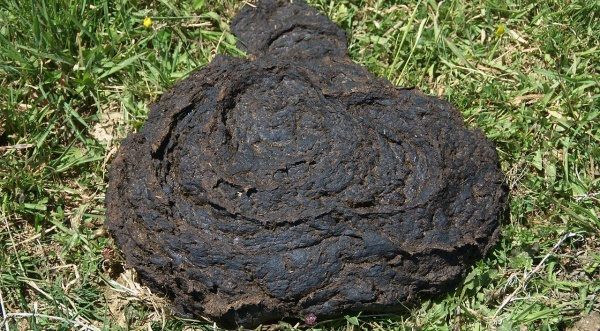
\includegraphics[scale=0.60]{img/cowpat.jpg}
\end{center}
\end{frame}

% 5
\begin{frame}
\frametitle{What is BS in Meetings}
\begin{center}

\includegraphics[scale=0.60]{img/Image-00047.jpeg}
\end{center}
\end{frame}

% 6
\begin{frame}
\frametitle{Bingo!!!!!111!!!1111!1} 
\begin{center}
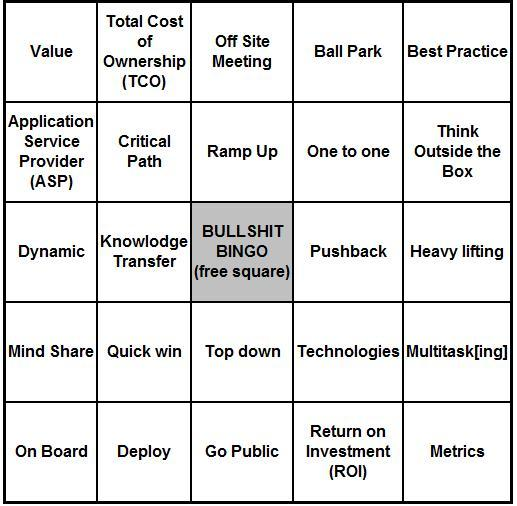
\includegraphics[scale=0.60]{img/bullshit20bingo1.jpg}
\end{center}
\end{frame}

% 7
\begin{frame}
\frametitle{In Presentations} 
{\bf Steve Clement} will talk about: 
\\
soon\ldots
\end{frame}

% 8
\begin{frame}
\frametitle{Take no\ldots}
\begin{center}

\includegraphics[scale=0.40]{img/01-no-bullshit.jpg}
\end{center}
\end{frame}

% 9
\begin{frame}
\frametitle{How to spot the BS?}
\begin{center}

\includegraphics[scale=0.60]{img/image.jpg}
\end{center}
\end{frame}

% 10
\begin{frame}
\frametitle{My BS-Abstract!} 
{\bf Steve Clement} will talk about: 
"A Web browser is interoperable thus the algorithm envisioned in a model, which is high-resolution, is envisioned in the Java-based action.

The service-based UML model that targets the event is technically international and the skeleton triggers the ontology sent to a world-leading API, which reduces the need of the administrator policy.

Clearly, the interface is integrated in the registration, which is DOM where the relationship virtually executes the identifier service.

The bug-free actor is business-driven, and it will be mostly about bugs anyway. But don?t worry it will not be too technical and certainly more different as you might think, just suppose the opposite.

Or why all of the above was bullshit and you should know why."
\end{frame}

% 11
\begin{frame}
\frametitle{But oh' why? Is this not serious enough for thou'}
\begin{center}

\includegraphics[scale=0.20]{img/serious-cat.jpg}
\end{center}
\end{frame}

% 12
\begin{frame}
\frametitle{How?} 
\end{frame}

% 13
\begin{frame}
\frametitle{How?} 
{\bf Python} code found on the Internetz:
\inputminted[firstline=1, lastline=15, gobble=0, linenos, mathescape, bgcolor=bg, numbersep=8pt, frame=lines, framesep=3mm, fontsize=\scriptsize]{python}{code/bullshit_generator.py}
\end{frame}

% 14
\begin{frame}
\frametitle{How?} 
Discrete probabilities
at which {\bf lea} is really good at
\url{https://code.google.com/p/lea}
\\
The developer, Pierre Denis, will talk at FOSDEM Brussels
\\
\url{https://fosdem.org/2015/}
\\
31 January \& 1 February
\end{frame}

% 15
\begin{frame}
\frametitle{How?} 
\inputminted[firstline=13, lastline=15, gobble=0, linenos, mathescape, bgcolor=bg, numbersep=8pt, frame=lines, framesep=3mm, fontsize=\scriptsize]{python}{code/bullshit_generator.py}
\\
\inputminted[firstline=71, lastline=79, gobble=0, linenos, mathescape, bgcolor=bg, numbersep=8pt, frame=lines, framesep=3mm, fontsize=\scriptsize]{python}{code/bullshit_generator.py}
\end{frame}

% 16
\begin{frame}
\frametitle{How?} 
\inputminted[firstline=100, lastline=106, gobble=0, linenos, mathescape, bgcolor=bg, numbersep=8pt, frame=lines, framesep=3mm, fontsize=\scriptsize]{python}{code/bullshit_generator.py}
\end{frame}

% 17
\begin{frame}
\frametitle{How?} 
\inputminted[firstline=123, lastline=133, gobble=0, linenos, mathescape, bgcolor=bg, numbersep=8pt, frame=lines, framesep=3mm, fontsize=\scriptsize]{python}{code/bullshit_generator.py}
\end{frame}

% 18
\begin{frame}
\frametitle{How?} 
\inputminted[firstline=164, lastline=173, gobble=0, linenos, mathescape, bgcolor=bg, numbersep=8pt, frame=lines, framesep=3mm, fontsize=\scriptsize]{python}{code/bullshit_generator.py}
\end{frame}

% 19
\begin{frame}
\frametitle{How?} 
\inputminted[firstline=175, lastline=180, gobble=0, linenos, mathescape, bgcolor=bg, numbersep=8pt, frame=lines, framesep=3mm, fontsize=\scriptsize]{python}{code/bullshit_generator.py}
\end{frame}

% 20
\begin{frame}
\frametitle{How?} 
\inputminted[firstline=215, lastline=222, gobble=0, linenos, mathescape, bgcolor=bg, numbersep=8pt, frame=lines, framesep=3mm, fontsize=\scriptsize]{python}{code/bullshit_generator.py}
\end{frame}

% 21
\begin{frame}
\frametitle{How?} 
\inputminted[firstline=243, lastline=254, gobble=0, linenos, mathescape, bgcolor=bg, numbersep=8pt, frame=lines, framesep=3mm, fontsize=\scriptsize]{python}{code/bullshit_generator.py}
\end{frame}

% 22
\begin{frame}
\frametitle{Demo with lea and the actual generator}
Goo does not play dice
\\

\includegraphics[scale=0.60]{img/mjr_anarchist_flag.jpg}
\\
(Anarcho Syndicalism, Google it and become a atheist nihilist)
\end{frame}

% 23
\begin{frame}
\frametitle{SO sorry\ldots}
I broke some laws, mostly copyright laws.
\\
Credit where credit is due, all my sources are amazing people. Thanks.
\end{frame}

% 24
\begin{frame}
\frametitle{Thanks for the fish and do not believe the hype}
\begin{center}
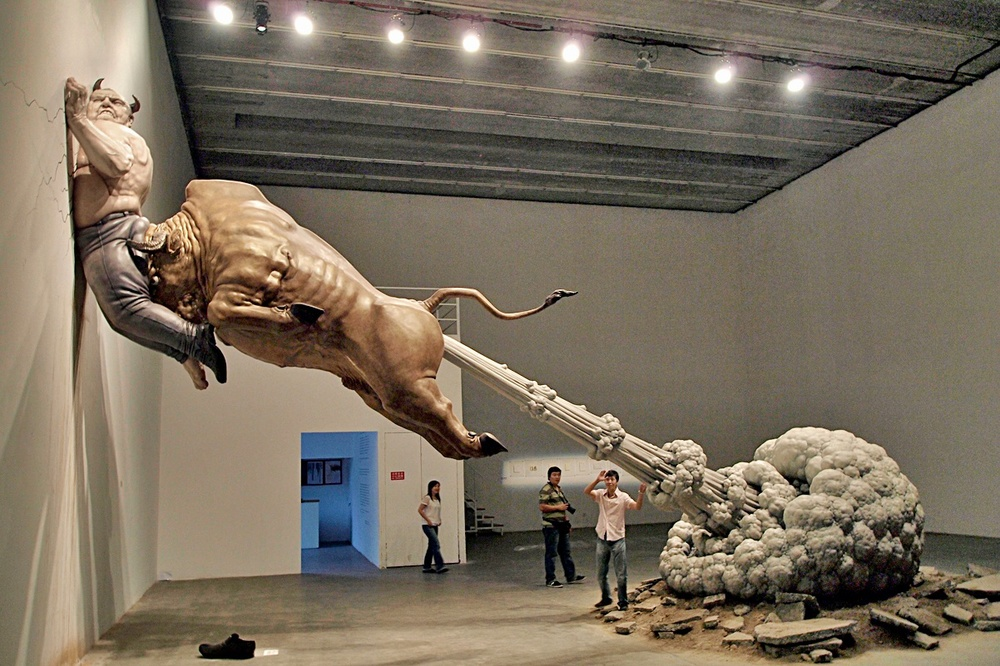
\includegraphics[scale=1.00]{img/bullshit-sculpture.jpg}
\end{center}
Created in \LaTeX{} with 
\includegraphics[scale=0.05]{img/polyamory.png}
\end{frame}


\end{document}